\Week{15}{More on Reed-Solomon Codes \& Applications}
In the unique decoding regime, to ensure that there is a unique codeword within the distance of $t$, we need  the error parameter $t<d/2$. What if $t=\lfloor\frac{d+1}{2} \rfloor$? In this case we know that 
there will be at least two code words in the hamming ball $B(y,t)$.  What can we do about it? How about obtaining a list of codewords that are within a distance of at most $t$ from the given erroneous message?
This leads us to the definition of  the List Decoding Problem which we discuss in this lecture.

\section{List Decoding \& Johnson's Bound}

\begin{definition}[\textbf{List Decoding Problem}]
Given a code $C\subset \Sigma^n$, a word $y\in \Sigma^n$, and a parameter $0<p<1$, compute a list $S$ of codewords in $C$ that are within a distance of $pn$ from $y$, i.e., output $S= B(y,pn)\cap C$.
\end{definition}

To talk about  efficient algorithms for  list decoding of a code $C$, it is also necessary to ensure that the set $S$ is not too large. Towards this, we set up the notion of List Decodable Codes:
\begin{definition}[{\bf List Decodable Codes}]
A code $C$ is said to be $(p,L)$ list decodable, if $\forall y\in \Sigma^n$, $|B(y,np)\cap C|\le L$.
\end{definition}

Thus, by definition, any $(n,k,d)_2$ code is $(\frac{\delta}{2},1)$ list decodable because $\frac{\delta}{2}$ is the unique decodability radius. Beyond $\frac{\delta}{2}$ it depends on the combinatorial stucture of the packing of words in the code - it is fathomable that the number of codewords at distance $\frac{\delta}{2}+\epsilon$ suddenly shoots up to exponential. The boundary at which it happens is something that we need to calculate. Hence, it is not clear  if $(p,L)$ list decodable codes exist. Following lemma gives an answer.
\begin{lemma}
\label{lem:list-exist}
Let $|\Sigma|=q, 0<p<1-1/q$. There is a code $C$ with rate $1-H_q(p)-1/L$ such that $C$ is $(p,L)$ list decodable, where $H_q(p)$ is the $q$-ary entropy function depending only on $p,q$.
\end{lemma}

The above lemma can be proved by a probabilistic argument by considering random codes in $\Sigma^n$. We will skip the proof. 
Though it tells us the existence of list decodable codes, we would prefer to know methods to find if a given code is list decodable. The answer is given by the Johnson bound which shows a possible bound for $p$ for which the ball of radius $pn$ centered at any word in $\Sigma^n$ contains more than one codeword interestingly at most $\poly(n)$ codewords.

\begin{theorem}[\textbf{Johnson Bound}]
Any $(n,k,d)_q$ code $C$ is $(J_q(\delta),qdn)$ list decodable, where
\[ J_q(\delta)= \left( 1-\sqrt{1-\frac{q}{q-1}\delta}\right)(1-\frac{1}{q})\]
and $\delta=d/n$, the relative distance.
\end{theorem}

An immmeidate corollary that we would like to derive is how useful it is. Let us apply it for $q=2$. It says, any binary linear code is linear sized list decodable if the number of errors made is at most $\half\left( 1-\sqrt{1-2\delta}\right)$ (you can check that this number is greater than $\half$ when $\delta$ is more than $\half$). 

One can ask the question whether the Johnson's bound is tight. The answer is yes - it can be shown (we dont provide the proof here) there exist linear codes with relative distance $\delta$ such
that we can find Hamming ball of radius larger than $J_q(\delta)$ with super-polynomially many codewords.

We will now prove Johnson's Bound for binary linear codes.

\begin{theorem}[\textbf{Johnson Bound for Binary Codes}]
Let $C$ be an $[n,k,d]_2$ code. Then every $y \in \zon$ and for $\frac{e}{n} < \half\left( 1-\sqrt{1-2\frac{d}{n}}\right)$, 
$$|B(y,e) \cap C| \le 2dn$$
\end{theorem}
\begin{proof}
The proof is by a double counting argument. Fix a $y \in \zon$. Let the ball $B(y,e) = B = \{c_1, c_2, \ldots c_\ell \}$. We need to prove that $\ell \le 2dn$. We will do translation first. Consider $c_i' = c_i - y$. This gives us words $B' = \{ c_1', c_2', \ldots, c_\ell' \}$ such that each has weight at most $e$ and the pairwise distance between them still remains the same because $d(c_i',c_j') = d(c_i-y,c_j-y)=d(c_i,c_j) \le d$. We will double count the sum of the pairwise distances in $B'$. Consider the sum:
$$S = \sum_{i < j} d(c_i',c_j')$$
One easy estimate for the summation is to use the distance bound for each pair to get a lower bound : $S \ge {\ell \choose 2}d$.
On one hand, let us consider the $n \times \ell$ matrix $M$ which has the words in $B'$ as columns. Let $w_r$ be the weight of the $r$-th row of this matrix. Counting the contribution of the columns to the sum $S$, whenever $i$-th and $j$-th column chosen to find the distance is having different entries in the $r$-th row of them, it contributes $1$ to the summation. The number of such pairs is $w_r(\ell-w_r)$. Thus we have, $S = \sum_{r=1}^n w_r(\ell-w_r)$. Let $w = \sum_r \frac{w_r}{\ell} = \frac{1}{\ell}\sum_r w_r$. Since $\sum_r w_r$ is counting the number of $1$s, which is also the sum of the weights of the $c_i'$s it is upper bounded by $e\ell$. Hence, $w \le \frac{1}{\ell}(e\ell) \le e$.
\begin{eqnarray*}
S = \sum_{r=1}^n w_r(\ell-w_r) = \sum_{r=1}^n \ell w_r-\sum_{r=1}^n w_r^2 \le \ell^2 w-\sum_{r=1}^n w_r^2
\end{eqnarray*}
To estimate the two terms, we will use Cauchy-Schwartz Inequality between the vectors, $(w_1, w_2, \ldots w_n)$ and $\left( \frac{1}{n}, \frac{1}{n}, \ldots, \frac{1}{n} \right)$. This gives,
$\left(\frac{\sum_{r=1}^n w_r}{n}\right)^2 \le \frac{\sum_{r=1}^n w_r^2}{n}$ and implies,

$$ S \le \ell^2w - \frac{\left(\sum_{r=1}^n w_r\right)^2}{n} \le \ell^2w - \frac{(\ell w)^2}{n} \le \ell^2\left(w -\frac{w^2}{n}\right)$$
Now we match it up with the lower bound:
$$ \frac{d\ell(\ell-1)}{2} \le \ell^2\left(w - \frac{w^2}{n}\right))$$
and this gives:
$$\ell \le \frac{dn}{dn-2nw+2w^2} \le \frac{2dn}{(n-2w)^2-n(n-2d)}
\le \frac{2dn}{(n-2e)^2-n(n-2d)}
\le 2dn$$
The last inequality follows from the assumption on $e$ which makes the denominator to be more than 1.
\end{proof}

There is also an alphabet-free version of Johnson bound, which we state for our information.
\begin{theorem}[{\bf Johnson Bound - alphabet free version}]
Any $[n,k,d]_q$ code with distance $d$ is $(\frac{e}{n},qnd)$-list decodable where $e \le n-\sqrt{n(n-d)}$.
\end{theorem}

\section{List-Decoding Algorithm for Reed-Solomon Codes}

We now describe an algorithm for list decoding of Reed-Solomon codes. To know what to expect, let us apply the alphabet-free version of Johnson's bound. Since $d=n-k+1$ for Reed-Solomon codes, this gives, that Reed-Solomon code has at most $O(n^3)$ codewords in any Ball of radius $e$ where $e < n - \sqrt{n(n-(n-k+1))}$. Thus, Reed-Solomon code is $(\rho,n^3)$-list-decodable where $\rho < 1 - \sqrt{R}$. Do efficient algorithms exist which can list decode Reed-Solomon codes? We first formulate the problem with the specific details of Reed-Solomon codes.

\begin{problem}[\textbf{List Decoding Reed-Solomon codes}]
Given $(\alpha_1, y_1),\ldots, (\alpha_n,y_n) \in \mathbb{F}^2$ and  $t\in \mathbb{N}$,  output all polynomials $p(x)$ of  degree at most $k-1$ such that
\[|\{i~|~p(\alpha_i)=y_i\}|\ge t \]
\end{problem}

Notice the change of notation. Rather than counting disagreements, we will count \textit{agreement} between evaluations of $p$ and the received vector $y$. The following remarkable result was proved in 1997, matching the Johnson bound for Reed-Solomon Codes.

\begin{theorem}[{\bf Guruswami-Sudan(1997)}]
There is a polynomial time algorithm (runs in time $\poly(n)$) that can solve the list decoding problem given a guarantee that $t > \sqrt{nk}$. 
\end{theorem}

Earlier than this, Sudan had described an algorithm which list decodes Reed-Solomon codes given the guarantee that $t > 2\sqrt{nk}$. The list size in this case is $\sqrt{\frac{n}{k}}$ which is
$\frac{1}{\sqrt{R}}$ for the error bound $n-\sqrt{2nk} = 1-\sqrt{2R}$. The smaller the rate $R = \frac{k}{n}$ of the code, the list size is high. Intutively, in this case the codewords will be more tightly packed and the list of words within the radius itself is higher. We will prove an even weaker version of the theorem, to list decode when the agreement is at least $(k+1)\sqrt{n}+1$. In fact the same algorithm, with a tighter analysis will give the required bounds as well.
\vspace{-4mm}
\paragraph{Extending Berlekamp-Welch Idea:} To get to the general case of the algorithm, let us quickly recall Welch-Berlekamp Decoder for Reed-Solomon Codes. The decoding algorithm, given $y \in \F_q^n$ first finds a pair polynomials $(N(x),E(x))$ s.t. $N(\alpha_i)/E(\alpha_i) = y_i$ holds for all $i \in [n]$ provided $E(\alpha_i) \ne 0$. And then output $N(x)/E(x)$ as a polynomial. This can be thought of as an interpolation problem.

Another way of thinking about the above task is that of finding a rational function\footnote{Rational function over a field $\F_q$ is the ratio of two polynomials defined over $\F$} $r(x) = \frac{f(x)}{g(x)}$ such that if $g(\alpha_i) \ne 0$, then $r(\alpha_i) = \frac{f(\alpha_i)}{g(\alpha_i)} = y_i$. And 
whenever $g(\alpha_i) = 0$, then $f(\alpha_i)=0$ as well and in this case we will allow $r(\alpha_i)$ to take any value. Keeping this view, the Berlekamp-Welch aim can be reformulated as {\em Find a rational function $r(x)$ such that $r(\alpha_i) = y_i$ for all $i$ whenever the denominator of the rational function evaluates to non-zero.} Indeed, thet theorem that we proved for Berlekamp-Welch decoding can be interpreted as : There exists a pair of polynomials $(N,E)$ exists with $deg(N) \le \frac{n+k}{2}$ and $deg(E) \le \frac{n-k}{2}$ such that $\frac{N}{E}(\alpha_i) = y_i$ holds whenever $E(\alpha_i) \ne 0$.
\vspace{-4mm}
\paragraph{\bf High level Idea:} 
Given a received word $y$, how do we output a set of polynomials which are "close" to $y$? One possibility is to output a product of those polynomials and then factorize it to get the individual polynomials. The above discussion gives the clue that we should be looking for more general algebraic objects to capture the data about the  evaluation of the polynomial. It turns out that 
It turns out we can use bivariate polynomials - we will do a curve fitting through the $i$ pairs $(\alpha_i,y_i)$ of points to get a bivariate polynomial $Q(x,y)$ and then factorise $Q$ to get the polynomials of the form $y-p(x)$. Fortunately, factorization of bivariate polynomials can be done in time polynomial in the degree.
\vspace{-4mm}
\paragraph{Example 1:}
We will take a more "curve fitting" view now. Consider the $n$ input pairs as points in a two-dimentional plane. We will try to fit in a bivariate polynomial that passes through all the points and try to strike a relationship between the different $p_i's$ and the bivariate polynomial. Consider the nine points on the plane.\\[-2mm]

\begin{minipage}{0.4\linewidth}
%\vspace{-4mm}
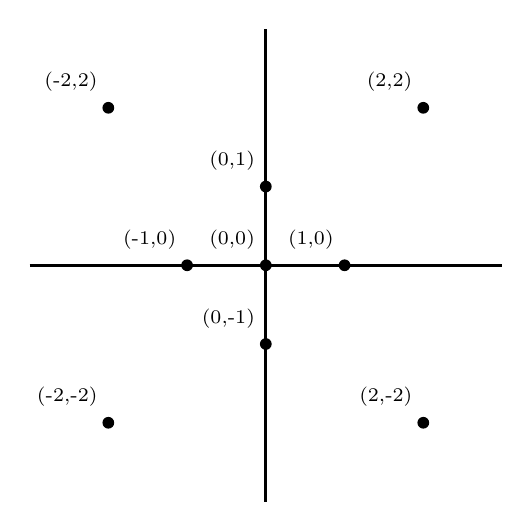
\begin{tikzpicture}
\tikzset{
    dot/.style 2 args={fill, circle, inner sep=1.5pt, label={#1:\scriptsize #2}}
}
\def\numberlist{(-2,2),(2,2),(0,1),(0,0),(-1,0),(1,0),(0,-1),(-2,-2),(2,-2)}
\foreach \pt in \numberlist
{
  \node[dot={100}{\pt}] at \pt {};
}
\draw[line width=1pt](0,-3) -- (0,3);
\draw[line width=1pt](-3,0) -- (3,0);
\end{tikzpicture}
\end{minipage}
\begin{minipage}{0.5\linewidth}
%\vspace{-3mm}
To obtain the polynomial in this case, define :
\begin{eqnarray*}
 Q_1(x,y) &=& x^2+y^2-1 \\
 Q_2(x,y) &=& x+y \\
 Q_3(x,y) &=& x-y
\end{eqnarray*}
Now the bivariate polynomial passing through all the nine points is: $Q(x,y) = Q_1 Q_2 Q_3$. Indeed, there are many challenges 1) which all points will be together in which $Q_i$ and 2) the bivariate polynomial passing through all the given points need not be unique. 
\end{minipage}

\paragraph{Example 2:} Given ${\alpha_1,\ldots, \alpha_n}\subseteq {\mathbb F}$, $y=(y_1,\ldots, y_n)\in {\mathbb F}^n$. Suppose there exist two degree $k-1$ polynomials $p_1(x), p_2(x)$ and $T\subset [n]$, $|T|=n/2$ such that
\[ y_i=\begin{cases} p_1(\alpha_i)~~\mbox{ if } i \in T\\ p_2(\alpha_i)~~\mbox{otherwise}. \end{cases}\]
The problem is to compute the polynomials  $p_1$ and $p_2$. 
Observe that $\forall i, y_i= p_1(\alpha_i)~\vee~y_i=p_2(\alpha_i)$, and hence
\[ \textrm{ For all $i \in [n]$, we have : } (y_i- p_1(\alpha_i))(y_i-p_2(\alpha_i)) = 0 \]
Now, if we define $Q(x,y)=(y_i- p_1(x))(y_i-p_2(y))$, then factorizing the polynomial $Q(x,y)$ would give us the answer. Since we do not yet know $p_1(x)$, and $p_2(x)$, we can try to find a polynomial
$Q$ from the data that $Q(\alpha_i,y_i)=0,~\forall i$, and then factorize $Q$. The algorithm can be described as follows.
\begin{enumerate}
\item Compute a polynomial $Q(x,y)$ of the form $y^2+ B(x)y+ C(x)$, where $B$ is a degree $k-1$ polynomial, and $C$ is a degree $2(k-1)$ polynomial such that  $Q(\alpha_i, y_i)=0,~1\le i\le n$. This can be done by solving for the coefficients of $Q(x,y)$, by the linear equations
\[ y_{i}^2+ B(\alpha_i) y_i+ C(\alpha_i)=0~~\forall i, \]
with coefficients of $B$, and $C$ as $3(k-1)$ unknowns. Solution exists if $n>3(k-1)$.
\item Factorize $Q(x,y)$ into $(y-p_1(x))(y-p_2(x))$, and output $p_1(x)$, and $p_2(x)$.
\end{enumerate}
As factorizing bi variate polynomials can be done in polynomial time, the above algorithm can be implemented in time $poly(n)$.  The following lemma sproves the correctness of the algorithm:
\begin{lemma}
For any polynomial $Q(x,y)$ omputed in Step 1 of the algorithm above, we have, $(y-p_1(x))|Q(x,y)$, and $(y-p_2(x))|Q(x,y)$.
\end{lemma}
\begin{proof}
We will prove that $(y-p_1(x))|Q(x,y)$, and the lemma follows by symmetry.
Consider $Q(x,y)$ as a polynomial in $y$ with  univariate polynomials in $x$ as coefficients, i.e.,
\[Q(x,y)=Q'(y)= Q_0+ Q_1y+ y^2.\]
We use the fact : if  $\beta$ is such that $Q'(\beta)=0$, we have $(y-\beta)|Q'(y)$. Hence, it is sufficient to show that $Q'(p_1(x))\equiv 0.$
We will show this by degree constraints. If for some $i$,~$y_i=p_1(\alpha_i)$, then $Q'(\alpha_i)=Q(\alpha_i, p_1(\alpha_i))=0$, and this is true for
at least $n/2$ of the index  $i$. But degree$(Q'(x)) \le 2(k-1)< n/2$, and hence it must be that $Q'(p_1(x)) \equiv 0$, and hence $(y-p_1(x))|Q'(y)$ and hence $(y-p_1(x))|Q(x,y)$.
\end{proof}

\paragraph{General Form - Bivariate Interpolation}
Learning from the examples, given a set of pairs ${(\alpha_i , y_i)}_{i\in [n]}$ we would fit them in an algebraic curve in the plane, that is, we would construct a bi-variate polynomial $Q(x,y)$ s.t. $Q(\alpha_i,y i) = 0$ for all $i \in [n]$. We first show existance and construction of $Q$.

\begin{lemma}[{\bf Bi-variate Interpolation}]
\label{lem:bivariate-interpolation} For every set of pairs ${(\alpha_i , y_i)}_{i\in [n]}$, there exists a non-zero
bivariate polynomial $Q(x,y)$ with $\deg_x(Q),\deg_y(Q) \le \sqrt{n}$ such that
$$Q(\alpha_i,y_i) = 0 \textrm{ for all $i \in [n]$ }$$
\end{lemma}
\begin{proof}
Let the polynomial $Q(x,y)$ be: 
$$Q(x,y) = \sum_{i,j \le \sqrt{n}} c_{ij} x^iy^j$$
Consider the $c_{ij}$s, the coefficients of $Q(x,y)$ as the unknowns and consider linear constraints among them represented by $Q(\alpha_i,y_i) = 0$ for all $i \in [n]$. Using the degree bound of $\sqrt{n}$ in each variable, the number of unknowns is $(\sqrt{n}+1)^2$. The number of constraints is $n$ making it an underdetermined consistent system (since zero polynomial is always a solution) and hence there are many solutions. We can compute the non-trivial solution for $Q(x,y)$ by solving this linear system.
\end{proof}

\paragraph{Sudan's Algorithm:}
We are now ready to describe the algorithm:

\begin{algorithm}
\label{alg:Berlekamp-Welch}
\caption{~:~Sudan's List Decoding Algorithm for Reed-Solomon Codes}
{\bf Input:} ${(\alpha_i , y_i)}_{i\in [n]}$ and $t > (k+1)\sqrt{n}$ \\
{\bf Output: } A list of polynomials $p_j(x)$ of degree $\le k$ such that $p_j(\alpha_i) = y_i$ for at least $t$ of the $i \in [n]$.
\begin{algorithmic}[1]
\State Find $Q(x,y)$ with $\deg_x(Q), \deg_y(Q) \le \sqrt{n}$.
\State Factorise $Q(x,y)$ to find an explicit list of factors of the form $y-p(x)$.
\State Output all those $p(x)$ such that 
$p(\alpha_i) = y_i$ for at least $t$ values of $i \in [n]$.
\end{algorithmic}
\end{algorithm}

Indeed, Step (1) in the algorithm can be done in $O(n^2)$ time since it is suffiicent to solve a system of linear equations for $n$ variables. Step (2) can be done in $\poly(n)$ time by a known efficient algorithm for bivariate factorization. Step (3) can be done in polynomial time, if we prove that the number of polynomials produced in Step (2) is bounded by $\poly(n)$. Hence it suffices to provide an upper bound to the size of the list, the value of $t$ and that completes the algorithm. How do we provide an upper bound to the list of polynomials. Indeed, the idea is that for each such polynomial, we argue that it contributes to the degree of $Q(x,y)$. Since there is an upper bound on the degree of $Q(x,y)$, we should have the upper bound on the list. The following lemma executes this plan.

\begin{lemma}
\label{lem:division-lemma}
 If $t > (\deg_x-1)+(k-1)(\deg_y-1)$, then $y-p(x) \mid Q(x,y)$.
\end{lemma}
\begin{proof}
View $Q(x,y)$ as a polynomial in $y$ with coefficient as polynomial expressions in $x$. 
$$Q(y) = Q_0(x)y^0+Q_1(x)y^1+....+Q_{\deg_y-1}(x)y^{\deg_y-1}$$
where $Q_i(x)$ is a polynomial in $x$ with degree $i$.
We use the simple algebraic property :
$Q(\beta) = 0$ implies that $(y-\beta) \mid Q(y)$.
Now, by our notation, $Q(p(x)) = Q(x,p(x))$. Hence, if $Q(p(x)) \equiv 0$ then $y-p(x)$ divides $Q(x,y)$ and we will be done.

Now we are left with the task of proving that $q(p(x)) \equiv 0$. This follows from degree considerations itself. 
Degree of the polynomial $Q(p(x))$ is atmost $d_x-1+(k-1)(d_y-1)$.
We show more than that many substitutions for $x$, which makes $Q(p(x))$ to be zero and hence conclude that $Q(p(x)) \equiv 0$.
Indeed, we already have them, $Q(p(\alpha_i)) = Q(\alpha_i,p(\alpha_i)) = 0$  for atleast $t$ indices and $t > d_x-1+(k-1)(d_y-1)$. Thus we conclude that, $Q(p(x)) \equiv 0$ and hence $y-p(x)$ divides $Q(x,y)$.
\end{proof}

This immediately implies that the number of such factors can atmost be equal to $\deg_y$. Thus the list size is bounded by $\sqrt{n}$ and $t > k\sqrt{n-1}$. But we can do better. Let us write down the constraints that we have for the above arguments to work.
\begin{eqnarray*}
\textrm{From Lemma~\ref{lem:bivariate-interpolation} :} & d_xd_y > n\\
\textrm{From Lemma~\ref{lem:division-lemma} :} & t > d_x-1+(k-1)(d_y-1)
\end{eqnarray*}
Thus, in the step $1$ of the algorithm, we can look for $Q$ with different degree constraints $\deg_x(Q)$ and $\deg_y(Q)$ such that the above constraints are satisfied. This gives a better list size if we choose $d_x = \sqrt{nk}$ and $d_y = \sqrt{\frac{n}{k}}$. The size of the list will be $\sqrt{\frac{n}{k}}$ and 
$t > (\sqrt{nk}-1) + (k-1)(\sqrt{\frac{n}{k}}-1)$. Hence if we insist that the agreement $t > 2\sqrt{nk}$ that satisfied the above constraint. By optimizing the choice of parameters, we can improve the required agreement constraint to $t >\sqrt{2nk}$. This is left as an exercise.

\begin{curiousity}[\textbf{Guruswami-Sudan Algorithm}]
To write the ideas required to improve the above agreement constraint to $t > \sqrt{nk}$ which matches (in relative to $n$) with the Johnson radius of $1-\sqrt{R}$ for Reed-Solomon codes.
\jsay{Yet to write about Guruswami-Sudan Algorithm}
\end{curiousity}

\begin{exercise-prob}[{\bf Scrambled Reed-Solomon Codes}]
% - Problem Set 4(See Problem~\ref{scrambled-rs})]
%\begin{show-ps4}{scrambled-rs}
Let $\{\alpha_1, \ldots , \alpha_n\}$ be distinct elements of $\F_p$ used to define a Reed-Solomon code $C : \F_p^k \to \F_p^n$. Assume that $k < \frac{n}{6}$. For this problem, assume the fact (used in class) that for a bivariate polynomial $Q(x,y)$, we can
find all its factors of the form $y-f(x)$.
\begin{enumerate}[(a)]
\item Suppose we sent two codewords corresponding to the polynomials $P$ and $P'$ (of degree $k-1$) but they got mixed up.Thus, we now have two lists $(\beta_1, \ldots ,\beta_n)$ and
$(\gamma_1, \ldots, \gamma_n)$ and we know for each $i \in [n]$:
$$\textrm{ \textbf{either} [$P(\alpha_i) = \beta_i$ and $P'(\alpha_i) = \gamma_i$] \textbf{or} [$P(\alpha_i) = \gamma_i$ and $P'(\alpha_i) = \beta_i$]}$$
Assuming that each co-ordinate is independently scrampled and we do not know which way each co-ordinate got scrambled, write down an algorithm to find out $P$ and $P'$. [Hint: First find $P+P'$ and $PP'$]
\item Now, suppose that instead of getting both the values $P(\alpha_i)$ and $P'(\alpha_i)$ for each $i$, we only got one value $\beta_i$, such that for each $i$ we either have $\beta_i = P(a_i)$ or $\beta_i = P'(a_i)$. Again, assume that each co-ordinate is independently scrampled and we do not know which way each co-ordinate got scrambled. We are given the promise that:
$$\frac{n}{3} \le \card{\{ i \in [n] \mid \beta_i = P(\alpha_i) \}} \le \frac{2n}{3} \textrm{ ~~~and~~~ } \frac{n}{3} \le \card{\{ i \in [n] \mid \beta_i = P'(\alpha_i) \}} \le \frac{2n}{3}$$
Design an algorithm to find out $P$ and $P'$. 
\end{enumerate}
%\end{show-ps4}
\end{exercise-prob}

\section{Algorithmic Applications of Reed-Solomon Codes}

In this lecture we present two applications of Reed-Solomon codes in algorithm design. The algorithmic models are very different and one uses the structure of the code alone and the second one uses the efficient unique decoding and list decoding algorithms for Reed-Solomon Codes.

\subsection{Communication Complexity}
As mentioned above, this application does not use the decoding algorithms for Reed-Solomon Codes, but rather it uses the  structure of the codewords. We will quickly introduce the communication complexity set up first.

Let $f : \zo^n \times \zo^n \to \zo$ be a Boolean function. The communication complexity model has two parties Alice and Bob - each holding a string in $\zon$ each, say $x \in \zo^n$ with Alice and $y \in \zon$ with Bob, and they want compute the function value $f(x,y)$. That is, at the end of the algorithm (which in the context of communication complexity, are called {\em protocols}) both the parties should know the result $f(x,y)$. The resource of computation here is the number of bits that they exchange\footnote{Alice and Bob have infinitel computational power an also knows each others computation strategy. What they do not know is each others $n$-bit input string.} expressed as a function of $n$. As in the case of algorithms, for a given function $f$, we would like to understand the number of bits exchanged, in the worst case over different $x$ and $y$, by the best protocol to compute the function. This is denoted by $CC(f)$.

Indeed, a trivial way to compute $f(x,y)$ is the following protocol: Alice sends $x$ across to Bob and Bob computes the function $f(x,y)$ and send the one bit answer back to Alice. This protocol takes $n+1$ bits of communication. This is independent of the function $f$. Hence, $CC(f) \le n+1$. A general question is whether we can do better than $n+1$, even asymptotically. \\[-10mm]

\paragraph{Examples:} 
Consider the function {\sc Par}$(x,y) = \bigoplus_{i=1}^n(x_i \oplus y_i)$. This function has a $2$-bit protocol which uses associativity of the $\oplus$ operator - Alice sends $b = \bigoplus_{i=1}^n x_i$ to Bob and Bob computes $\left( b \bigoplus \left( \oplus_{i=1}^n y_i \right) \right) $ and returns the bit $b$. Thus, $CC(\textrm{\sc Par}) = 2$ and {\sc Par} is an easy function for this model of computation.

Let us take a second example. Consider $\textrm{\sc Eq}(x,y) = \land_{i=1}^n \left( x_i = y_i \right)$. That is, to check if the two strings $x$ and $y$ are the same or not. A moments thought might convince you informally that one should probably expect this function to be harder in communication complexity model. Indeed, it is true - $CC(\textrm{\sc Eq}) = n+1$. This requires proof though, and communication complexity offers quite a number of exciting proof techniques for showing upper and lower bounds. We leave that discussion aside since that is a digression at the moment.

We get to a randomized communication complexity model, where Alice and Bob also has a source of shared randomness (unbiased coin flipes). Indeed, the requirement is that over a good fraction of outcomes of the random bits that they choose, the answer given by the protocol must be equal to $f(x,y)$. More formally, if $\calP$ is the protocol:
$$\forall x,y ~\Pr_{r \in \zo^m} [ \calP(x,y,r) = f(x,y) ] \ge \half+\epsilon$$
Indeed, as in the case of randomized algorithms, one can imagine protocols which produces only one sided error, and protocols with two sided error (in which case, we want $0 < \epsilon \le \half$).

We attempt on a randomized algorithm for {\sc Eq}$(x,y)$ function. A trivial attempt first. Suppose Alice and Bob chooses a random $i \in [n]$ (using their common randomness). Alice sends across $x_i$ and Bob checks if $x_i = y_i$, if yes, Bob declares that the function value is $1$ and otherwise $0$. Let us analyse this randomized protocol. Indeed, if $x = y$, then the protocol never errs - no matter which $i$ is chosen, $x_i = y_i$ will be satisfied. Hence it is a one-sided error randomized protocol. Suppose $x \ne y$. A moment of through will reveal the worst case setting where $x_i \ne y_i$ for exactly one $i \in [n]$ and the strings match at other indices. In this case, the probability of success is $\frac{1}{n}$. Note that we cannot afford to repeat the algorithm linear number of times since that increases the communication complexity to linear (which the trivial protocol also achieves anyway).


\paragraph{Using Reed-Solomon Codes to Design Randomized Protocols for {\sc Eq}$(x,y)$}:
So a natural question is whether Alice and Bob can transform their inputs to some longer strings, where the above randomized algorithm (of choosing an index at random and checking for equality at the index for both their inputs) can be done. An intutive  idea would be that, if there is one index in which the strings $x$ and $y$ differ, then there must be many differences in the new strings which gets caught by the randomized algorithm with noticable (constant) probability. Codes indeed have this natural property and as we will demonstrate below, Reed-Solomon codes, just does the job.

The idea is quite simple - Both Alice and Bob encodes their inputs as Reed Solomon Code words of a $[N,K,N-K+1]_q$ where $q \ge N$ and $K=n$. We will choose the blocklength $N$ appropriately for the required error parameter. Let $\epsilon > 0$ be the target error. Thus, as a part of the encoding, Alice and Bob have polynomials $P_x$ and $P_y$ respectively of degree at most $K-1$ each. The codewords are evaluations of the polynomials on the elements in $\F_q$. Let $c_x, c_y \in \F_q^N$ be the codewords such that any $\alpha \in \F_q$ forms an index to the codeword, and $c_x[\alpha] = P_x(\alpha)$ and $c_y[\alpha] = P_y(\alpha)$.
The protocol is same as described in the previous paragraph which we write in formal form below.

\begin{algorithm}
\label{alg:communication-complexity}
\caption{~:~Communication Protocol for {\sc Eq}$(x,y)$ using Polynomials}
{\bf Input:} Alice has $x \in \zon$ and Bob has $y \in\zon$ \\
{\bf Output: } Both Alice and Bob must know {\sc Eq}$(x,y)$.
\begin{algorithmic}[1]
\State Using the Reed-Solomon Code $[N,K,N-K+1]_q$, Alice and Bob independently computes $c_x = C(x)$ and $c_y = C(y)$ respectively (both in $\F_q^N$).
\State Choose an $\alpha \in \F_q$ uniformly at random from a common random source.
\State Alice sends $b = c_x[\alpha] \in \F_q$ to Bob. Bob checks if $b = c_y[\alpha]$. If yes, Bob declares {\sc Eq}$(x,y)$ is $1$, and $0$ otherwise.
\end{algorithmic}
\end{algorithm}

We argue the success probability. Suppose $x = y$, then $C(x) = C(y)$ as well. Hence no matter which $\alpha$ is chosen in step 2, Bob will end up declaring {\sc Eq}$(x,y) = 1$. Suppose $x \ne y$, then, we want to analyse the number of differnet $\alpha \in F_q$ such that $c_x[\alpha] = c_y[\alpha]$. Indeex, consider any such an $\alpha$. We know that $P_x(\alpha) = P_y(\alpha)$. Hence, $\alpha$ is a root of the univariage polynomial $P_x - P_y$, which is of degree at most $n-1$. Hence, the number of such $\alpha$s is bounded by $n-1$. Thus, the error probability,
$$\Pr_{\alpha \in \F_q} \left[c_x[\alpha] = c_y[\alpha]\right] = \Pr_{\alpha \in \F_q} \left[P_x(\alpha) = P_y(\alpha) \right] \le \frac{n-1}{q} \le \frac{n}{q}$$
Hence, if we have target error probability to be at most $\epsilon$, then we have to choose $q=N \ge \frac{n}{\epsilon}$. The communication complexity is $O(\log \frac{n}{\epsilon})$. If $\epsilon$ is a constant, then we have an $O(\log n)$ cost protocol for {\sc Eq}$(x,y)$. Compare this with $\Omega(n)$ lower bound that we mentioned in the beginning of this section. Thus, in the setting of communication complexity, randomization is provably more powerful and these protocols cannot be derandomized without incurring linear cost overhead.

One final remark about this applicatin is that it is a bit artificial since we did not use any property about the code such as distance and decoding algorithms. In the next section, we present a "real" application of codes.

\begin{exercise}[\textbf{Protocol using Hadamard Codes}]
Come up with a protocol for {\sc Eq}$(x,y)$ function with cost $O(\log n)$ bit of communication, using Hadamard Codes.
\end{exercise}

\subsection{Self-Correcting Algorithms for Permanent}

The driving question for this section is the following possibility  : Can we have a mechanism for tranforming our programs which may fail on small fraction of inputs (that is, the algorithm works correctly on most of the inputs) into programs that are usually correct into randomized programs that are always correct, with high probability. Notice that we want to do this without using any details of the program that we are tranforming and hence should be done in a blackbox way. Interestingly, this can be done for certain problems, in fact, in general for algorithms whose task is to evaluate implicit polynomials. We make this more precise as we go further.

Let $p$ be a prime. We will consider the algorithmic problem of computing the determinant of an $n \times n$ matrix $A= \left(A_{i,j}\right)_{i,j=1}^{n}\in \F_p^{n \times n}$. Computing the determinant by highschool method involves recursively computing the cofactors and then adding up them. A quick analysis shows that this recursion follows the recurrence $T(n) = nT(n-1)+n$ which gives a runtime of $2^{O(n\log n)}$. A different formulat for the determinant which is derived by using the properties\footnote{such as exchanging two columns will change sign of the determinant, such as having two columns identical results in zero-value for determinant etc. See \href{https://en.wikipedia.org/wiki/Leibniz\_formula\_for\_determinants}{here} for more details.} of the determinant - is the Leibniz formula for determinant is
\begin{equation}
\det(A) = \sum_{\sigma\in S_n}{\sf sign}(\sigma)
\prod_{i=1}^n A_{i,\sigma(i)}
\label{eqn:leibnis}
\end{equation}
where $S_n$ is the set of all permutations on $n$ symbols, and ${\sf sign}$ is the sign function of a permutation, i.e ${\sf sign} (\sigma) = -1$ if the number of inversions in $\sigma$ is odd, and~$1$ otherwise.

Even Leibniz formula does not help in computing the determinant of a given $n \times n$ matrix efficiently. The algorithm which explcitly computes the summands in Leibniz formula will take time $O(n!) = 2^{O(n \log n)}$ time.
This is impractically difficult for large $n$. 
Instead, the determinant can be evaluated in $O(n^3)$ operations by forming the $LU$ decomposition of $A$ as $A = LU$. In this case, $\det A = (\det L)(\det U)$ and the determinants of the triangular matrices $L$ and $U$ are simply the products of their diagonal entries. The $LU$ decomposition is computed by using Gaussian elimination. 

A close cousin of the determinant is called the {\sf Permanent} function of a matrix. The expression for this function is similar when we write in the Leibnis form - by dropping the  ${\sf sign}$ function from the definition of determinant function. That is, for an $n \times n$ matrix,
\[{\sf perm}(A) = \sum_{\sigma\in S_n}\prod_{i=1}^n A_{i,\sigma(i)}.\]

Indeed, given the matrix $A$, computing the permanent does not yield to an algorithm. An immeidate approach is to follow the above expression explicitly, but as observed this requires at least $2^{O(n \log n)}$ time. In the case of determinant, it had special alternating properties which makes the Gaussian elimination work and hence gave an $O(n^3)$ algorithm. But in the case of permanent, there is no useful property like that. In fact, it is conjectured that permanent cannot be computed in polynomial time. In his seminal paper, Valiant showed that computing ${\sf perm}_n$ is polynomial time equivalent to counting the number of
satisfying assignment of a Boolean formula. Noting that even testing whether there is a satisfying assignment for a given formula or not is considered to be a difficult problem ($\NP$-complete), and counting the number of satstying assignments is harder. \\[-8mm]

\paragraph{Characterstic of the Field Matters:}
We should remark about finite fields since that is what we are going to work with. Consider the case when $p=2$. Over $\F_2$, notice that $+$ and $-$ operators yield the same result, and hence sign can be dropped from determinant. In other words, over $\F_2$, computing the determinant is same as computing the permanent of a matrix with entries from $\F_2$. Hence, the Gaussian elimination computes the permanent of the matrix itself over $\F_2$. Indeed, even the above reduction due to Valiant requires $p$ to be large. \\[-8mm]

\paragraph{Randomized Algorithms for {\sf perm$(A)$}?:}
A natural question to ask is whether we can have randomized algorithms for computing the permanent of a matrix. To make the model precise, given a matrix $A$, the algorithm $\calR$ can toss random bits $r \in \{0,1\}^m$, but should provide the guarantee:
$$\Pr_{r \in \zo^m} \left[ {\sf perm}(A) = \calR(A,r) \right] \ge \half+\epsilon$$

It is worth noting that having efficient randomized algorithms for computing the permanent will immediately yield efficient randomized algorithms for testing satisfiability of a given formula $\phi$. This is currently unknown, and is conjectured to be not true. Hence, \textit{it is very unlikely that the task of computing permanent of a given matrix can be performed through an efficient randomized algorithm}. This last statement is what we rely on in this lecture.\\[-8mm]

\paragraph{Algorithms with Correct-on-Most-Inputs type guarantee:}
Note that the above lower bound  for ${\sf perm}$  is as worst-case lower bound, and still does not eliminate the possibility of a polynomial time algorithm $A$ such that $A$ computes permanent correctly for a constant fraction of matrices $B \in F_p^{n \times n}$. 

\subsubsection{Applying Unique-Decoding Regime : Gimmel-Sudan Algorithm}

Continuing from the previous discussion, we ask the following question: \textit{Is there  algorithm $\calA$ such that $\calA$ runs in time $\poly(n)$ and computes ${\sf perm}(A)$ for at least $\alpha$ fraction of input matrices $B \in \F_p^{n \times n}$, for a constant $\alpha>0$?}
We use the unique decoding regime of Reed-Solomon codes, in order to answer the above question as NO, by showing that if there is such an algorithm, then there is an efficient randomized algorithm which computes permanent on all matrices with high probability.

\paragraph{Random Tranlations of Matrices:} We demonstrate the idea by presenting a simpler case when $\alpha = 1-O(1/n)$. Let $p > n$. This one does not use codes. 
\begin{theorem}[\textbf{Lipton}]
If $\calA$ is an algorithm that computes ${\sf perm}$ for all but a $\frac{1}{3(n+1)}$ fraction of matrices in $\F_p^{n \times n}$, 
then there is a randomized polynomial time algorithm computing ${\sf perm}$ on all matrices $B \in \F_p^{n \times n}$, with probability at least $2/3$.
\end{theorem}

\begin{proof}
Suppose we have an algorithm $\calA$, that computes ${\sf perm}$ for all but a $\frac{1}{3(n+1)}$ fraction of matrices in $\F_p^{n \times n}$. Our aim is to design a randomized algorithm that computes ${\sf perm}$ on all input $B\in \F_p^{n \times n}$ matrices with probability at least $2/3$. For this, consider an input matrix $B\in \F_p^{n \times n}$, define the matrix
\[D(x) = B+ xC\]
where  $C$ is a matrix chosen uniformly at random from $\F_p^{n \times n}$ and $x$ is an indeterminate. The first observation is that since $B$ is fixed as the input matrix, for any substitution of $t \in \F_p$, $D(t)$ is unformly distributed over the set of matrices in $\F_p^{n \times n}$. In particular, since $p > n$, for $i \in [n+1]$, $D(i)$ is also uniformly distributed in $\F_p^{n \times n}$.

The matrix $D$ has variable $x$ appearing in various entries. Consider $P(x)= {\sf perm}(D(x))$. Notice that $P(x)$ is a polynomial of degree at most $n$ in $x$ - since any permutation can multiply at most $n$ appearances of the variable $x$ in the expression in Equation~\ref{eqn:leibnis}. If we somehow have access to this polynomial $P(x)$, then $P(0) = {\sf perm}(D(0)) = {\sf perm}(B)$. Hence, $P(0)$ is the answer that we are looking for. Thus the strategy now is to look for ways to compute $P(x)$.

Let $Q(i)= \calA(D(i))$, $i=1,\ldots ,n+1$. Note that $P(x)$ is   a uni-variate polynomial of degree at most $n$, and $P(x)={\sf perm}(B)$. By the property of algorithm $\calA$, and since $D(i)$ is uniformly distributed in $\F_p^{n \times n}$, we have:
\begin{eqnarray}
\forall i\in[n+1]~~\Pr_{C \in \F_p^{n \times n}} \left[Q(i)\neq P(i)\right] \le \frac{1}{3(n+1)} \\
\label{eqn:unionbound}
\textrm{Hence, by union bound, }\Pr_{C \in \F_p^{n \times n}}\left[\exists i \in [n+1],~ Q(i)\neq P(i)\right]\le 1/3\\
\textrm{Hence,~}\Pr_{C \in \F_p^{n \times n}}\left[\forall i \in [n+1],~ Q(i) = P(i)\right] \ge 2/3
\end{eqnarray}
That is, with probability at least 2/3 over the choice of $C \in \F_p^{n \times n}$, we have the evaluations of the polynomial $P$ (of degree at most $n$) in $n+1$ points. Thus, we get $n+1$ points through which the polynomial $P(x)$ must pass through. Let them be $(x_0,y_0),(x_1,y_1), \ldots, (x_n,y_n)$. We can directly write the polynomial as:
$$ P(x) = \sum_{i=0}^n y_i \left(\prod_{\substack{j=0\\j \ne i}}^n \frac{(x-x_i)}{(x_j-x_i)} \right) $$
And, $P(0)= {\sf perm}(B)$ is the required output. In fact, this gives a direct formula for the permanent.
$${\sf perm}(B) = \bigsum_{i=1}^{n+1} \calA(D(i)) \left(\prod_{\substack{j=1\\j \ne i}}^{n+1} \frac{i}{(i-j)} \right)$$ 
where, all operations are in $\F_p$ and since $p \ge n+1$, $[n+1]$ is identified with the corresponding elements in $\F_p$ (in this case $\Z_p$). We describe the randomized algorithm for ${\sf perm}$:

\begin{algorithm}
\label{alg:rand-algo-perm1}
\caption{~:~Lipton's Randomized Algorithm for {\sf perm} using $\calA$}
{\bf Input:} $B \in \F_p^{n \times n}$.
{\bf Output: } ${\sf perm}(B)$.
\begin{algorithmic}[1]
\State Choose $C \in  \F_p^{n \times n}$ uniformly at random.
\State Let $D(x)= B+xC$.
\State Run $\calA$ on $D(1), \ldots, D(n+1)$ to obtain values $y_1= \calA(D(1)), \ldots, y_{n+1}=\calA(D(n+1))$.
\State Interpolate to get a polynomial $Q$ with $\deg(Q) \le n$ such that $\forall i \in [n+1], Q(i)=y_i$.
\State Output $Q(0)$.\end{algorithmic}
\end{algorithm}

By the argument above, 
$\Pr_{C \in \F_p^{n \times n}}\left[ Q\equiv P \right] \ge 2/3$
and hence the correctness follows.
\end{proof}

\paragraph{Strengthening Lipton's Theorem beyond $\frac{1}{3n+1}$ error bound:}
From Lipton's theorem, we concluded that it is unlikely to have a deterministic algorithm computing permanent on all but $\frac{1}{3n+1}$ fraction of matrices in $\F_p^{n \times n}$. But then, can there be an efficient algorithm which does signifinantly worse than this - that say, computes correctly on all but $\frac{1}{4}$ fraction of matrices in $\F_p^{n \times n}$. In this section, we will use Reed-Solomon codes in order to achieve a similar reduction upto an error bound of $\half-\epsilon$.

\noindent \textbf{An instructive attempt:} A natural attempt is ensure we have evaluations of $D(x)$ on more points via the algorithm $\calA$. But how much more? Let us call this number $N$. We view $(P(1), \ldots, P(N))$ which are the correct evaluations as a \textit{codeword} in an $[N,n,N-k+1]$ Reed-Solomon code, where $p \ge N \ge n+1$ and view the error made by the algorithm as the corruptions made by the channel. Given the above set of parameters, instead of using interpolation, we could use the Berlekamp-Welch decoding algorithm to get the polynomial $P(x)$ by correcting at most $(N-k+1)/2$ errors in the received word $(Q(1), \ldots, Q(N))$. Thus we can allow $\calA$ to err on at most $(N-k+1)/2$ of the matrices in $\{D(i)~|~i=1,\ldots, N\}$. But then if the $D(i)$s where independent, then situation would have been easy - it suffices if error probability of $\calA$ is be at most  $(N-k+1)/2N$, then we can recover the polynomial $P(x)$ from the values $(Q(1), \ldots, Q(N))$ by applying Berlekamp-Welch decoding algorithm. Thus, setting $N= \frac{n}{2\epsilon}$ for $\epsilon>0$ would have given the desired bounds. 

But unfortunately, $D(i)$s are not independent. Hence, we ended up using union bound (in Equation ~\ref{eqn:unionbound}) to deduce that with constant probability, all the evaluations are going to be correct. As discussed above, here the constraints are different: we cannot expect the algorithm to succeed on all of the instances for any setting of the random bits. The best that we can hope for is to get the correct answers on $\alpha N$ of the input points. We need to establish such a concetration of the probability. For this, we need to design $D$ with more indepednence. It turns out that pairwise independence would suffice, and apply Chebyshev’s inequality to conclude that with high probability, the number of correct answers
is indeed close to $\alpha N$. \cite{GS92} implemented exactly that.

\begin{theorem}[\cite{GS92}]
For any $\epsilon > 0$, if $\calA$ is an algorithm that computes ${\sf perm}$ for all but a $\left(\half-\epsilon\right)$ fraction of matrices in $\F_p^{n \times n}$, 
then there is a randomized polynomial time algorithm computing ${\sf perm}$ on all matrices $B \in \F_p^{n \times n}$, with probability at least $2/3$.
\end{theorem}

\begin{proof}
We construct (by careful sampling from $\F_p^{n \times n}$ a domain $D \subseteq \F_p^{n \times n}$) parametrized by a single variable
$x$ (that is, the points in the domain $D$ are given by $\{D(x)| x \in \F_p \})$, such that $D$ satisfies the following properties:
\begin{description}
\item{\sf Property 1:} The function $P(x) = {\sf perm}(D(x))$, is a univariate polynomial of degree at most $2n$ in $x$. The end-result that we want will be $P(0)$. So our aim will be to compute the polynomial $P(x)$ in explicit form.
\item{\sf Property 2:} With high probability, $\calA$ computes ${\sf perm}$ on approximately the same fraction of inputs from the
domain $D$ as from the domain $\F_p^{n \times n}$.
\end{description}

Notice that the two properties are contradictory - first one requires the domain $D$ to be \textit{nicely structured} while the second one requires that sampling from $S$ should look like \textit{random sample} of $\F_p^{n \times n}$. It is an interesting puzzle whether we can achieve both simultaneously. It turns out that if we choose $D$ to be {\em pairwise independent samples} it achieves best of both worlds. This is the main idea proposed \cite{GS92}.\\[-8mm]

\paragraph{Construction:} Let $B \in \F_p^{n \times n}$ be the input matrix. Let $S,T \in \F_p^{n \times n}$ chosen uniformly at random and define :
$$D(x) \defn \{ Sx^2 + Tx + B \}$$
As in the case of Lipton's theorem, define $P(x) = {\sf perm}(D(x))$. 
For a given $S$ and $T$, define the family as:
$$\calD_{S,T} = \{ D(x) \mid x \in \F_p \}$$

\noindent We argue the properties required. To see {\sf Property 1} $P(x)$ is, by definition, a polynomial in degree at most $2n$. Right away, we have that $P(0) = {\sf perm}(B)$. To see, {\sf Property 2}, we claim that for any substitution $i$ for $x$, $D(i)$ is distributed in $\F_p^{n \times n}$ uniformly, over the choice of matrices $S$ and $T$. We need to conclude about the fraction of inputs from the domain $D$. We are aiming to use a Reed-solomon code of parameters $[N,K,N-K+1]_p$ over the field $\F_p$. Choosing $K=2n$, and $N$ will be fixed later - we need to get at least $\frac{N-2n+1}{2}$ co-ordinates in the codeword right by the algorithm $\calA$ to apply this framework. The following lemma achieves that with appropriate choice of parameters.

\begin{lemma}
\label{lem:GS-Lemma}
Consider $N$ elements from the set $D_{S,T}$ above:
$$\Pr \left[ \begin{array}{c}
\textrm{$\calA$ computes {\sf perm} correctly on at least}\\
\textrm{$\left(N \left(\half+\epsilon\right)-c\sqrt{N}\right)$ samples} 
\end{array}
\right] \ge 1-\frac{1}{c^2}$$
\end{lemma}
To apply the lemma, let $e$ be the number of elements in the sample set $S$ of $N$ samples in $D$, in which the algorithm $\calA$ makes an error. If we choose the number of samples to be $N = (\frac{c}{\epsilon}+n)^2$, then with probability at least $1-\frac{1}{c^2}$, we have that 
\begin{eqnarray}
e \le \left(\frac{c}{\epsilon}+n\right)^2\left(\half-\epsilon\right)+ c\left(\frac{c}{\epsilon}+n\right) & \le & \half\left(\frac{c}{\epsilon}+n\right)^2 - \left(\frac{c}{\epsilon}+n\right) \epsilon n \\
& \le & \frac{N}{2}\ - cn - \epsilon n^2 < \frac{N-2n+1}{2}
\end{eqnarray}
The last inequality holds for large enough $n$. Hence, we can apply Berlekamp-Welch decoding algorithm directly to get the polynomial $P$ and evaluate $P(0)$ to get the ${\sf perm}(B)$ correctly. Thus, $c \ge 2$ will achieve a success probability of $\frac{2}{3}$ and the algorithm runs in time $\poly(N)$, which is $\poly(n,\frac{1}{\epsilon})$.

\begin{proof}[\textit{\bf Proof of Lemma~\ref{lem:GS-Lemma}}]
For any fixed $i$, $D(i)$ is uniformly distributed over $\F_p^{n \times n}$ (Prove this as an exercise !). We prove the following indepedence claim.

\begin{claim}
The family $\calD = \{ D(x) \mid x \in \F_p \}$
is pairwise independent.
\end{claim}
\begin{proof}
Recall the definition of $D(x) \defn Sx^2 + Tx + B$ where $S$ and $T$ are chosen uniformly at random from $\F_p^{n \times n}$. To show pairwise independence, 
For any two matrices $S',T' \in \F_p^{n \times n}$, and $a,b \in \F_p$, we need to prove that:
$$\Pr_{S,T} \left[ (D(a) = S') \land (D(b) = T') \right] = \frac{1}{p^{2n^2}}$$
This follows by observing that for each entry of the matrix $(i,j)$, there is exactly one degree 2 polynomial $p_{ij}(x)$ such that $p_{ij}(0) = B_{ij}$ and $p_{ij}(a) = S_{ij}$ and $p_{ij} = T_{ij}$ (since degree 2 polynomial is uniquely determined by three evaluations).
\end{proof}

Now the lemma follows from the claim below about a tail inequality for pairwise independent random variables. A careful application of Chebychev inequality (using the fact that variance of the sum is the sum of variances, when the random variables are pairwise independent) gives:

\begin{lemma}
If $S$ is a set of $N$ samples from the pairwise independent space $D \subseteq \F_p^{n \times n}$. For any $I : U \to \zo$. Then for any positive constant $c$:
$$\Pr \left[ \left| \E_{x \in U} I(x) - \E_{x \in D} I(x) \right| \ge \frac{c}{\sqrt{N}}\right] \le \frac{1}{c^2}$$
\end{lemma}
To apply the lemma, we define $I(x)$ to be the indicator random variable of when the algorithm $\calA$ computes ${\sf perm}(D(x))$ correctly. Indeed, $\E_{x \in U} I(x) = \half+\epsilon$ and the above lemma estimates the tail of the distribution using Chebychev inequality.
\end{proof}
\end{proof}

\begin{curiousity}[{\bf Reselient Algorithms for Computing Polynomials}]
The framework that we discussed is applicable to the problem of correcting programs that compute multivariate polynomials over large finite fields and not just computing the permanent polynomial. This gives an efficient procedure to transform any program that computes a multivariate polynomial $P(x)$ correctly on a $1/2+\epsilon$ fraction of its inputs ($\epsilon > 0$) into a randomized program that computes $P(x)$ correctly on every input with constant probability. In fact, this is the result proved by \cite{GS92} and the argument presented in this lecture is a corollary of their proof.
\end{curiousity}

\subsubsection{Applying List-Decoding Regime : Cai-Pavan-Sivakumar Algorithm}

Note that the \cite{GS92} breaks down if the original algorithm $\calA$ makes at least $1/2+\epsilon$ fraction of errors. However, by applying list decoding algorithms we can improve this  - that is, $\calA$ can be allowed to err on at most $1-\frac{1}{n^c}$ where $c$ is a constant.

\begin{theorem}[\textbf{Cai-Pavan-Sivakumar} \cite{CPS99}]
Let $c>0$ be a constant. Suppose there is a deterministic polynomial time algorithm $\calA$ computing ${\sf perm}$ over $\F_p$ for all $n$, and $p\ge 9n^{2c+2}$ correctly on at least $1/n^{c}$ fraction of the inputs from $\F_p^{n \times n}$, then there is a randomized polynomial time algorithm computing ${\sf perm}$ on all matrices $B \in \F_p^{n \times n}$, with probability at least $2/3$.
\end{theorem}
\begin{proof}
For the ease of presentation, we will also assume an upper bound on $p \le n^{c'}$ for a constant $c' > c$. Now we get on to the proof. Let $\calA$ be the algorithm as mentioned in the premise of the lemma, computing permanent correctly for at least $\alpha \ge 1/n^c$ fraction of the matrices in $\F_p^{n \times n}$, i.e.,
\[\Pr_{B\in \F_p^{n \times n}}[\calA(B) = {\sf perm}(B)] \ge 1/n^c.\]
Consider $B \in \F_p^{n \times n}$. Let $B_{1,1}, B_{2,1}, \ldots, B_{n,1}$ where $B_{i,1}$ is the $(n-1)\times (n-1)$ matrix obtained by deleting $i$th row and $1$st column of $B$.  Note that ${\sf perm }(B)= \sum_{i=1}^n b_{i,1}{\sf perm}(B_{i,1})$,
where $B= (b_{i,j})_{i,j=1}^n$. Let $\delta_i(x)$ denote the delta function for $i\in[n]$ i.e.,
\[\delta_i(x)= \begin{cases} 1~~~\mbox{ if }i=x, \\ 0~~~\mbox{ if }i\neq x. \end{cases}\]
Note that $\delta_i(x)$ is a degree $n$ polynomial. Let
\[\alpha(x)= \prod_{i=1}^n (x-i),\]
and
\[D(x)= \sum_{i=1}^{n}\delta_{i}(x)B_{i,1}+ \alpha(x)(S+ x T)\]
where $S,T \in \F_p^{(n-1) \times (n-1)}$ chosen uniformly at random. Define $P(x):= {\sf perm}(D(x))$, then $P(x)$ is a degree $(n+1)(n-1)=n^2-1<n^2$ polynomial. Note that if we knew $P(1), \ldots, P(n)$ we can determine permanent of $B$ as:
$$ {\sf perm}(B) = \sum_{i=1}^n b_{i1}P(i) $$
Thus, our aim now is to compute the polynomial $P(x)$ as in the earlier case. We need to ask for evaluations of $P(x)$ by using $\calA$ on $D(x)$ for different substitutions for $x$ other than $\{1,2, \ldots n\}$. Let 
\[D= \{D(a)~|~a=n+1,\ldots, p\}.\]
Suppose the matrices $S,T$ are chosen are uniformly and independently at random from $\F_p^{(n-1) \times (n-1)}$, then $D(i)$ is distributed uniformly from $\F_p^{(n-1) \times (n-1)}$. Moreover set $D$ is a set of pairwise independent family of matrices in $\F_p^{(n-1) \times (n-1)}$ over the choice of $S$ and $T$. Using this, the following lemma can be proved by applying the Chebyshev's inequality. We will defer the proof of the Lemma to the end and proceed with the proof of the Theorem.

\begin{lemma}
\label{lem:success}
With probability at least $1-\frac{1}{(p-n)\alpha^2}$, algorithm $\calA$ correctly computes ${\sf perm}$ on at least $\frac{\alpha}{2}$ fraction of the matrices in $D$.
\end{lemma}

We use the lemma with the following modelling of the situation. Let us define the graph of a polynomial $f$ is needed,
\[G_f := \{(i,f(i))~|~i=1,\ldots, p\}.\]
Let $S= \{(i, \calA(D(i))~|~i=n+1,\ldots, p\}$, then by  Lemma~\ref{lem:success} we have $|S\cap G_P|\ge \frac{\alpha}{2}(p-n)$ with probability at least $1-\frac{1}{(p-n)\alpha^2}$.  Now that idea is to obtain a list $T$  of polynomials of degree less than $n^2$ such that
$|S\cap G_f|\ge \frac{\alpha}{2}(p-n)$ applying Sudan's list decoding algorithm with input $\{(i, A(D(i)))~|~i=n+1,\ldots ,p\}$. However we need an  upper bound on the size of such a list:
\begin{lemma}[{\bf bound on the size of the list}]
\label{lem:listsize}
There are at most $\frac{3}{\alpha}$ polynomials $f$ such that $$|S\cap G_f|\ge \frac{\alpha}{2}(p-n)$$
\end{lemma}
Assuming the Lemma, we complete proof of Theorem as follows.
Now, apply $\calA$ to $D(i)$, for $i=n+1,\ldots, p$, then we know that $(\calA(D(n+1)), \ldots, \calA(D(p)))$ agrees with $(P(n+1), \ldots, P(p))$ on at least $\frac{(p-n)}{2n^c}$ of  the co-ordinates with probability $1-\frac{1}{(p-n)\alpha^2}$. Notice that, 
$$\frac{(p-n)}{2n^c} > \sqrt{2(p-n)n^2} \textrm{~~since $p \ge 9n^{2c+2}$~}$$
Thus, the number of polynomials $f$ of degree at most $n^2-1$ such that $(A(D(n+1)), \ldots, A(D(p)))$ and  $(f(n+1), \ldots, f(p)))$ agree on at least $\sqrt{2(p-n)n^2}= \sqrt{2Nk}$ coordinates is at most $\frac{3}{\alpha} \le 3n^c$, where $N=p-n, k=n^2$. Hence, the word $(P(n+1), \ldots, P(p))$ can be seen as a codeword in an $[L, k, L-k+1]_p$ Reed Solomon code. Thus, we can apply Sudan's list decoding algorithm in the input $\{ (i,  A(D(i))~|~i=n+1,\ldots, p\}$, with $t=\frac{(p-n)}{2n^c} > \sqrt{2Lk}$.
Let $T$ be the list of polynomials of degree at most $k-1=n^2-1$ output by Sudan's algorithm. We have $|T|\le \frac{3}{\alpha} \le 3n^c$. Moreover, we know that $T$ contains the polynomial $P(x)$. \\[-8mm]

\paragraph{Identifying the Correct Polynomial from the codword list $T$:} All we need to do now is  to separate  $P(x)$ from the  rest of the polynomials in $T$. As any two polynomials in $T$ can have a common value on at most $n^2-1$ points in $\F_p$, there are at most $9n^{2c}(n^2-1)$ points in $\F_p$ such that more than two polynomials in $T$ agree on each of those points.  Since  $p\ge 9n^{2c+2}$,  there is a $v\in\F_p$ such that $f(v)\neq g(v)~~\forall f\neq g\in T$. By a Brute force search and evaluation of polyomials in the list on each element in $\F_p$, we will find out this $v \in \F_p$ explicitly\footnote{This is where we use the upper bound of $p$ in terms of $\poly(n)$.}. 

Now, if we have access to ${\sf perm}(D(v))$, then $P(x)$ can be isolated from $T$, and in turn we can compute ${\sf perm}(M)$. The only thing that remains to be done is computing ${\sf perm}(D(v))$. Note that $D(v)$ is an $(n-1)\times (n-1)$ matrix, and hence we can recursively apply the whole process with $D(v)$ as the starting matrix instead of $M$.
\begin{eqnarray*}
\Pr~[\textrm{ Algorithm Errs }] & \le & \Pr~[ \exists i : \textrm { Algorithm Errs at Recursive Level $i$ } ] \\
& \le & \sum_{i=1}^{n} \Pr~[\textrm{ Algorithm errs at level $i$ }] \\
& \le & \sum_{i=1}^n \frac{1}{(p-n)\alpha^2} \le \frac{n}{(p-n)\alpha^2} \le \frac{n^{c+1}}{9n^{2c+2}} \le \frac{1}{9n^{c+1}} 
\end{eqnarray*}

Summarizing, the  randomized algorithm for ${\sf perm}$  can be described as follows:

\begin{algorithm}
\label{alg:rand-algo-perm1}
\caption{~:~Cai-Pavan-Sivakumar's\cite{CPS99} Randomized Algorithm for {\sf 
perm} using a given algorithm $\calA$ such that for a constant $c$ : $\Pr_{B \in \F_p^{n \times n}}[\calA(B)= {\sf perm}(B)]= \alpha \ge 1/n^c$.
}
{\bf Input:} $B \in \F_p^{n \times n}$.\\
{\bf Output: } ${\sf perm}(B)$.
\begin{algorithmic}[1]
\State  Define $D(x) \defn \sum_{i=1}^n \delta_i(x)M_{i,1}+\alpha(x)(S+xT)$
choosing $S,T \in \F_p^{(n-1) \times (n-1)}$ uniformly and independently at random.
\State Let $Q(i):= A(D(i))$, $i=n+1,\ldots, p$.
\State Apply Sudan's list decoding algorithm  with input $\{(i, Q(i))~|~i=n+1,\ldots, p\}$, $t=\frac{(p-n)}{2n^c}$.
Let $T$ be the list of polynomials of degree at most $n^2-1$ computed by Sudan's algorithm.
\State Compute $v\in \F_p$ such that $ \forall~f\neq g \in T$, $f(a)\neq g(a)$. Since there is such an $a$, this can be done by a brute force search.
\State  Recursively compute the value $b:={\sf perm}(D(v))$. (Note that $D(v)$ is an $(n-1)\times (n-1)$ matrix, hence the dimension of the matrix goes down by one at each level of recursion)
\State Find an $f\in T$ such that $f(v)=b$ (i.e., $f$ has to be $P$ with high probability, why?).
\State Output $\sum_{i=1}^n b_{i,1}f(i)$. 
\end{algorithmic}
\end{algorithm}

\noindent To complete the proof, we prove Lemma~\ref{lem:success} and Lemma~\ref{lem:listsize}.

\begin{proof}[{\em \textbf{Proof of Lemma~\ref{lem:success}}}]
 For $i=n+1, \ldots, p$, let $Z_i$ as 1 if $A$ succeeds on $D(i)$ and $0$ otherwise. Notice that $\E[Z_i] = \alpha$. Define the average random variable:
$$Z = \frac{1}{p-n}\sum_{i=n+1}^p Z_i$$
Let us calculate $\E[Z]$. By linearity, this is $\frac{1}{(p-n)}\sum_{i=n+1}^p \E[Z_i]$. This gives, $\E[Z] = \alpha$. We apply Chebychev inequality:
\begin{eqnarray*}
\Pr\left[Z \le \frac{\alpha}{2}\right] & = & \Pr\left[Z-E[Z] \le -\frac{\alpha}{2}\right] \\
& \le & \Pr\left[\left|Z-E[Z]\right| \ge \frac{\alpha}{2}\right] \le \frac{{\sf Var}[Z]}{\left(\frac{\alpha}{2}\right)^2}
\end{eqnarray*}

Since the random variables $Z_{n+1},\ldots, Z_p$ are pairwise independent, ${\sf Var}[Z] = \frac{1}{(p-n)^2}\sum_{i=n+1}^p {\sf Var}[Z_i] \le \frac{p-n}{4}$ by using the trivial upper bound for variance\footnote{Any 0-1 random variable has variance at most $\frac{1}{4}$. This is consequence of a more general theorem called 
\textit{Popoviciu's inequality}. Let the random variable be $X$ and $a \le X \le b$, then ${\sf Var}[X] \le \frac{(b-a)^2}{4}$. A quick proof when $a=0$, $\E[X^2] = \E[XX] \le \E[bX]$. If $z = \E[X]$. We have ${\sf Var}(X) = \E[X^2] - (\E[X])^2$. ${\sf Var}(X) \le cz - z^2$. This is maximised at $z = \frac{b}{2}$ and the maximum value is at most $\frac{b^2}{4}$.} Thus we have:
$$\Pr\left[Z \le \frac{\alpha}{2}\right] \le \frac{1}{(p-n)\alpha^2}$$
\end{proof}

\begin{proof}[{\em \textbf{Proof of Lemma~\ref{lem:listsize}}}] Suppose there are more than $\frac{3}{\alpha}$ polynomials $f$
polynomials of degree$<n^2$ such that $|S\cap G_f|\ge \frac{\alpha}{2}(p-n)$. Let $T$ be the set of $\lceil \frac{3}{\alpha} \rceil$ many of them. Then we have
\begin{eqnarray*}
p-n &\ge& |\cup_{f\in T} S\cap G_f| \ge \sum_{f\in T}|S\cap G_f| - \sum_{f\neq g\in T}|S\cap G_f \cap G_g|~~\mbox{by inclusion-exclusion principle}\\
&=& |T|\frac{\alpha}{2}(p-n)- {|T|\choose 2} (n^2-1);~~\mbox{since $f$, $g$ are of degree at most $n^2-1$, $|G_f\cap G_g|\le n^2-1$}.\\ 
&=& \frac{|T|}{2}\left(\alpha(p-n)- (|T|-1)n^2\right)
\end{eqnarray*}
Since $|T|=\lceil\frac{3}{\alpha} \rceil$, then $|T| < \frac{3}{\alpha}+1$, and $|T|\ge \frac{3}{\alpha}$, then substituting these to the above equation appropriately,
\begin{eqnarray*}
p-n& > & \frac{3}{2\alpha}\left(\alpha(p-n)- \frac{3}{\alpha} n^2 \right) \\
&=& \frac{3}{2}(p-n) - \frac{9n^2}{2\alpha^2} = (p-n) + \half\left((p-n) - \frac{9n^2}{\alpha^2}\right)\\
\end{eqnarray*}
If we show that the second term is positive, we have a contradiction. This is true, because $p > 9n^{9c+2}$ and hence $p-n > \frac{9n^2}{\alpha^2}$. Thus we get a contridiction and hence there can be strictly less than $\frac{3}{\alpha}$ many polynomials $f$
polynomials of degree$<n^2$ such that $|S\cap G_f|\ge \frac{\alpha}{2}(p-n)$. and this conludes the proof of Lemma~\ref{lem:listsize}.
\end{proof}
This concludes the presentation of the Cai-Pavan-Sivakumar Algortihm.
\end{proof}